In the following sequence diagrams, we describe exactly the interactions between the key
actors our system. It is important to note that most of the interaction between the
user and system is facilitated by the browser. The user, through filling forms and button
clicks, instructs the browser which requests to make to the system.
In turn, the system communicates with the database to request the desired data,
takes any required actions, and delivers the data to the browser for presentation to the user. \\

\begin{figure}
\centering
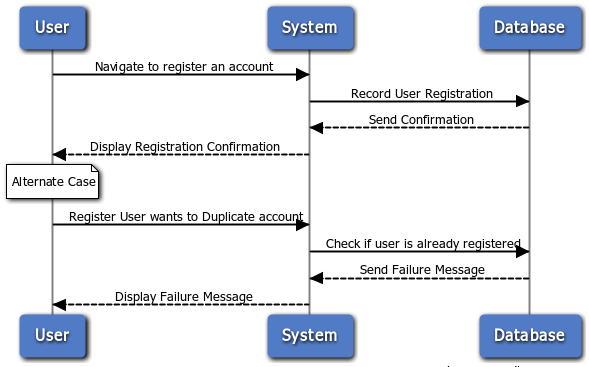
\includegraphics[width=5.5in]{./img/uc1.png}
\caption{See UC-1 on page \pageref{UC-1}. When the user navigates to the login/register accounts
page, this use case
is triggered. The system makes it necessary to have an account before using
Paramount Investments leagues. The System then takes the information that the
user has input and sends them to the database, which then sends it back to the
system to display on the screen to the user. If the system finds that the user that is
registering with the same credentials as an existing account, the system throws up
an error appropriately.}
\end{figure}

\begin{figure}
\centering
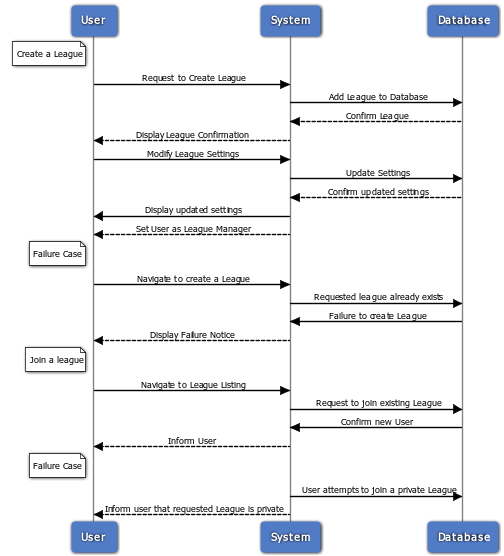
\includegraphics[width=5.5in]{./img/uc2.png}
\caption{See UC-2 on page \pageref{UC-2}. This use case is triggered when the user navigates
to the create league page.
The user requests the system to create a league, which then sends appropriate
data to the database. Once the data is stored successfully, the database sends a
confirmation back to the system, which then displays an appropriate message to the
user. If the user wants to join a league, the user requests the system appropriately,
which then sends the data to the database regarding the right league and if
successful sends the confirmation to the user.}
\end{figure}

\begin{figure}
\centering
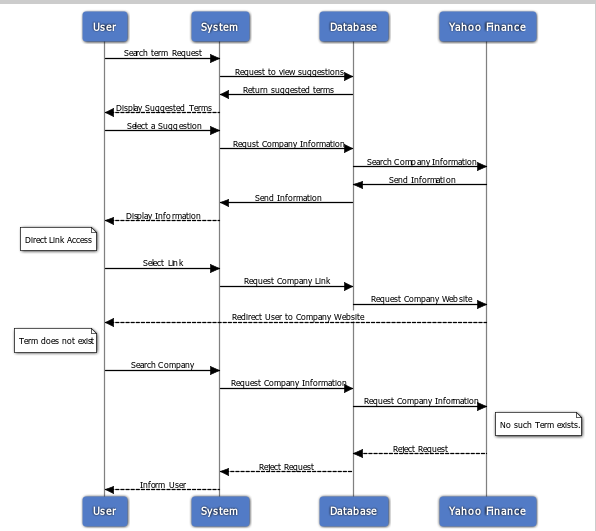
\includegraphics[width=5.5in]{./img/uc3.png}
\caption{See UC-3 on page \pageref{UC-3}. When the user navigates to the research
stock page, this use case is triggered. The
user specifies to the system exactly what market data they would like to view. If
the user wants to research off the company’s website, then user will click on the
hyperlink present in the system. If the user wants to view the data through the
interface that Paramount Investment Provides, the system then pulls information
from the Yahoo Finance API and then sends it back to the system to display to the
user.}
\end{figure}

\begin{figure}
\centering
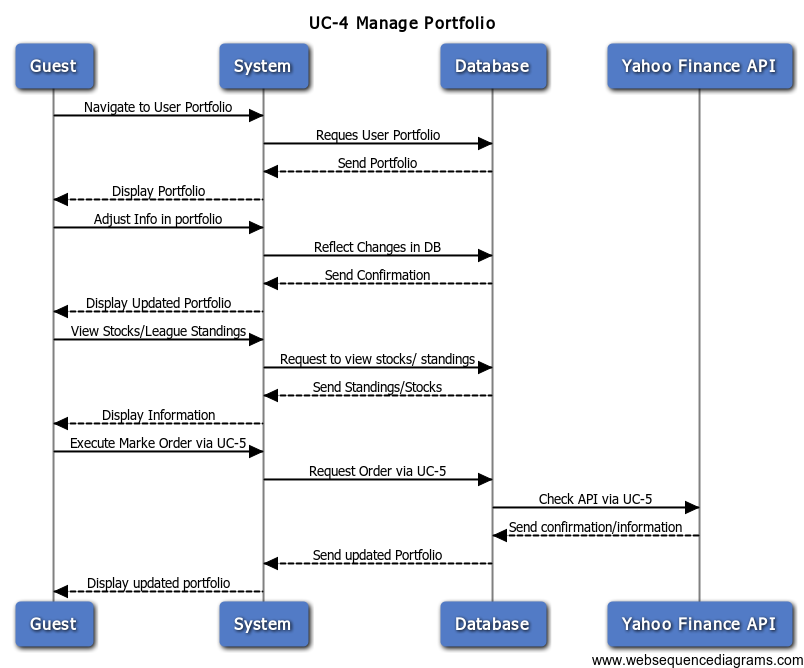
\includegraphics[width=5.5in]{./img/uc4.png}
\caption{See UC-4 on page \pageref{UC-4}. This use case is triggered when the user
goes to his/her own portfolio page. The
user navigates to the view portfolio page. The system then requests the database
to retrieve the user’s information. Once the database sends this data back to the
system, the system displays it to the user. The user is now free to modify aspects of
his/her portfolio. Once the user is finished modifying/updating their portfolio, the
system will send the changes to the database, which will then store the information
and save it.}
\end{figure}

\begin{figure}
\centering
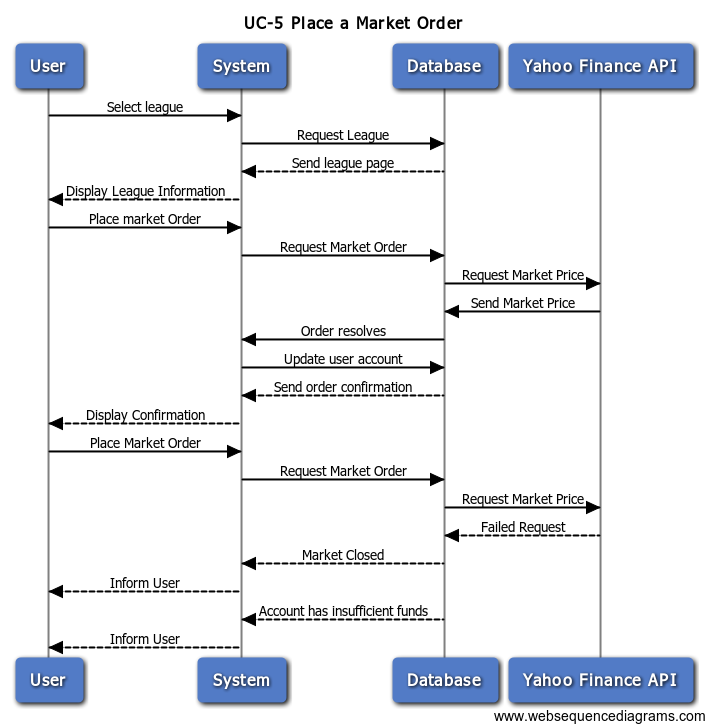
\includegraphics[width=5.5in]{./img/uc5.png}
\caption{See UC-5 on page \pageref{UC-5}. This use case is triggered when the
user goes to place a market order in the place
order page. The user selects a league to place the order into. The system then
displays the information to the user, who then requests to place a market order.
The system then queries to Yahoo Finance API to retrieve information about the
stock prices. The system then takes that information and processes it with what
the user wants to do. If the order is completed successfully, it is appropriately
displayed.}
\end{figure}

\begin{figure}
\centering
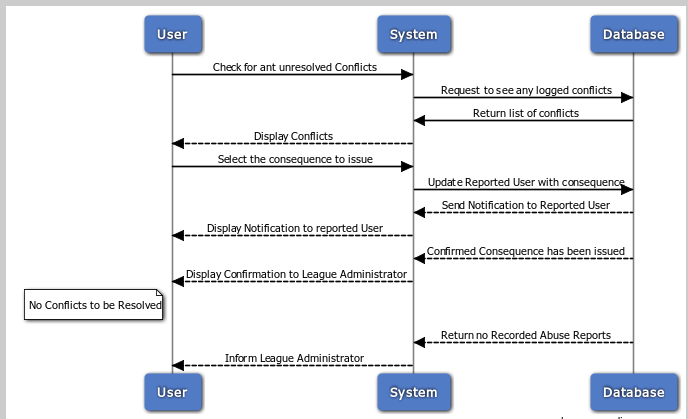
\includegraphics[width=5.5in]{./img/uc6.png}
\caption{See UC-6 on page \pageref{UC-6}. This use case is triggered when the
administrator of the website/ league wants
to take action. The system first checks if the user logging in has administrative
privileges in their respective group. If so, the system then looks in the database
to check for any logged conflicts. If there are unresolved conflicts, the database
returns them and then user can then view the conflicts. If there are no conflicts to
be resolved, then display so appropriately to the administrator/logged in user.}
\end{figure}

\begin{figure}
\centering
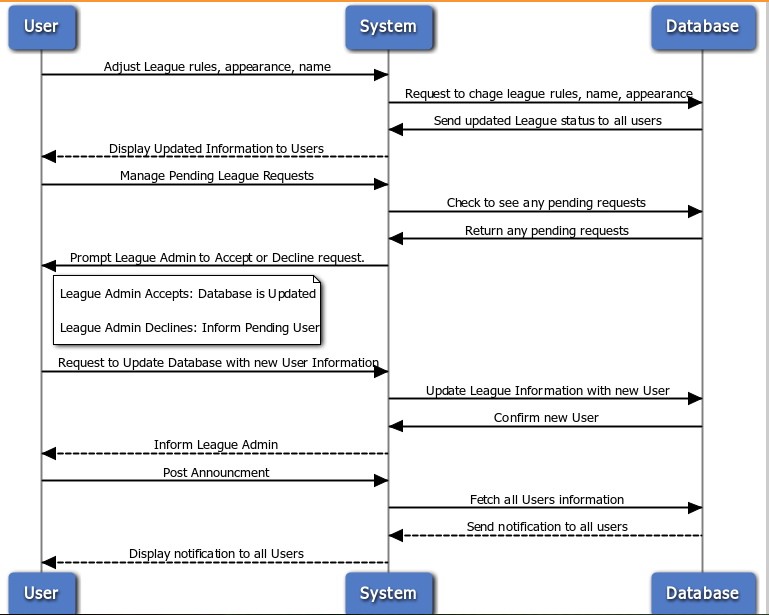
\includegraphics[width=5.5in]{./img/uc7.png}
\caption{See UC-7 on page \pageref{UC-7}. This use case is triggered when the
manager of a league wants to change the league
settings. The system first checks to see if the user that is logged in, is the league
manager and if so, the grants the user privilege to change league settings. The user
then requests to change the league settings. The system retrieves the league data
and modifies it as the user has requested.}
\end{figure}

